\documentclass[11pt, oneside]{article}   	
\usepackage{geometry}                		
\geometry{letterpaper}                   		
\usepackage{graphicx}												
\usepackage{amssymb}
\usepackage{natbib}
\usepackage{filecontents}


\title{Response to Eric C. Anderson Comprehensive Question}
\author{Patrick Barry}						

\begin{document}
\maketitle
\section{Written Essay}
	Coalescence is the process of coming together. All genetic variation arises through mutation. This
simple fact is a powerful one. It means that if we look far enough back in time all genetic variation that 
we see in the current population arose from some common ancestor. If we consider two gene lineages 
and look back in time tracing their ancestry, when we reach their most recent common ancestor (MRCA)
they are said to have coalesced. The rate of coalescense is determined by both the number of lineages that
are present and the population size. Each geneology consists of two types of information; time til 
coalescence and topology.

	As population geneticist we use variation in allele frequencies to ask and (hopefully)
answer a variety of questions about the relative importance of different genetic and demographic processes 
(e.g. population size change and genetic drift, selection, migration, mutation, and recombination)
responsible for this variation. We rely on simplified models such as the Wright-Fisher or Moran models to 
test hypotheses. The coalescent process is a particularly powerful approach for a number of tasks including
creating null distributions to test hypotheses, estimating parameters themselves, and evaluate statistical methods. 

	If a certain demographic process is suspected of happening, coalescent simulations can give us a null distribution
for  expectations of parameters of interest. Let's take a population bottleneck for example. 
During a bottleneck both the number of alleles and the heterozygosity decrease. 
The rate of loss of alleles is much higher as a result of rare alleles being lost, and those rare alleles 
contribute minimally to the heterozygosity. So the heterozygosity observed should be greater to than the 
heterozygosity expected under mutation drift equilibrium. We can collect data on a population suspected to
have undergone a bottleneck but we need some way of describing the null distribution of heterozygosity under
mutation-drift equilibrium. The coalescent allows this. This is what the program BOTTLENECK \citep{Piry1999}
does. In this case we used a very simple model, but the null expectation could be a more elaborate model that incorporates 
recombination, migration, etc. Coalescence forms the basis for approximate Bayesian computation
where random genealogies are simulated under certain model assumptions. Parameters of the simulation
can be altered until the simulated data resemble real data. Forward in time can provide expectations in the future
under a given model, so they may be more useful in describing what may happen under certain models.
Forward in time simulations can give us a better understanding of what happens depending on the initial 
conditions  \citep{Rosenberg2002}. The likelihood of fixation and the rate of fixation of different polymorphisms
are types of questions that are much more straightforward with forward in time simulations.  

	The parameter $\theta$ (Watterson's estimator) is pervasive in population genetics. In the n-coalescent it is 
defined in terms of the effective population size ($N_e$) and time. The trouble is that if we want to make inference
on time we often only have a collection of polymorphisms with which we can measure divergence. Rescaling 
the equation in terms of the mutation rate ($\mu$) such that we no longer can make inference on the parameter
$\theta$, $\theta=4N_e\mu$ for diploids and $2N_e\mu$ for haploids. So either $4N_e$ or $2N_e$ generations
have passed for mutation to occur. The scaling is somewhat arbitrary if adjustments are 
made to other parameters in the model. Once $\theta$ is estimated if we know either 
of the other two parameters we can infer the other. Estimating
$N_e$ is difficult, often confidence intervals contain infinity as an upper bound. Estimates of the mutation 
rate could be made from a variety of sources including fossils (ancient DNA). 

	Similarly, often new analytical approaches need to be tested where the demographic and genetic
processes shaping the genetic variation are known. This can provide information on the relative precision
and bias that accompanies their inference with the approach considered. A fundamental difference between the 
coalescent and forward in time simulations is that the coalescent considers genes that are sampled, whereas
forward in time simulations model alleles in the population for the entire population. If mutations are selectively neutral 
then the mutational process can be considered separate from the genealogical process. 
Resultantly, genealogies can be simulated and mutations can be added to the branches 
after \citep{Rosenberg2002}. Not keeping track of the entire population, just the sampled genes means that
simulations can be much more efficient. 

	Coalescent theory because it deals with describing genetic polymorphisms deals with mutation in a 
clear and straightfoward manner. Recombination can also be incorporated into the coalescent process. 
The main result of recombination is that within a sequence there can be different genealogical 
trees \citep{Rosenberg2002}. The effects of drift, migration, reproductive isolation can all be incorporated
into the coalescent process. The effect of selection have been incorporated into the coalescent process with the 
effects of recombination \citep{Hudson1988}, but \citet{Rosenberg2002} suggests that its incorporation is 
not as straightforward. This is a result of the fact that a major assumption of the coalescent process is that
lineages come together randomly. If selection is acting, some genotypes or lineages will disproportionately 
contribute to the next generation in a non-random fashion. 


\section{Practical Part}
1. Assume $N_e = 200$. Use Hudson?s program makesamples (also called ms) to simulate a single, 
non-recombining region of genome under this scenario. Simulate 20 copies (like 10 sampled diploids) 
from each of the two populations and force ms to give you 10 segregating sites on the segment. 
Write down the command line you would use. (Hint: you will need the -s, -I, and -ej options for this.)\\

\noindent
We would run the command:

\noindent
./ms 40 1 -t 0.0064 -s 10 -I 2 20 20 -ej 0.025 2 1 \\

\noindent
This runs the program ms creating 40 samples (20 diploids) for one rep. With flags 
for segregating sites, subpopulation sizes and time since the split.

\begin{description}
	\item[] -t is $\theta=4N_0\mu$, which will use $N_0$ of 200, and $\mu$ of $10^{-8}$.
	\item[] -s the number of segregating sites is set to 10
	\item[] -I is set to have 2 populations of twenty samples each
	\item[] -ej specifies that at time 0.25 all individuals from subpopulation 2 are placed
		in subpopulation 1
\end{description}

So where did the 0.25 come from as the time? This I am not sure I completely understand, so 
it is in all likelihood wrong. We know that $\theta=4N_0 \mu$, so if we assume $N_0$ to 
be 200 and we are scaling by 4, then we have $200/800$ for a time. 

\noindent
The output looks like:

\noindent
./ms 40 1 -t 0.0064 -s 10 -I 2 20 20 -ej 0.0.25 2 1\\ 
61269 32785 1897\\
//\\
prob: 4.3468e-22\\
segsites: 10\\
positions: 0.0175 0.2445 0.2630 0.3504 0.4040 0.5507 0.5733 0.5850 0.6163 0.9712 \\
0010000001
0010010010
0010010110
0010000000
0010000000
1101100000
0010000000
0010000000
0010000000
0010000000
0010010110
0010000000
0010010010
0010000000
0010010110
0010000000
0010010110
0010010110
0010000001
0010000000
0010000000
0010000000
0010000000
0010010010
0010010010
0010000000
0010000000
0010000000
0010010010
0010000000
0010010110
0010000000
0010000000
0010000000
0010010010
1101101000
1101100000
0010010010
0010010010
0010000000\\
\noindent\\
We have created 40 sequences with each of the 10 segregating sites show. \\

2. Now, simulate 10,000 such recombining sequences and record the distribution of 
the number of segregating sites (out of 10) in which the polymorphism is observed 
in the sample from both populations.\\

I am going to make the assumption you mean non-recombining sequences here, as ($\rho$) was not mentioned above. To 
do this we will run the same command but we are going to change the number of reps to 10,000. We will run the code:\\
\noindent\\
./ms 40 10000 -t 0.0064 -s 10 -I 2 20 20 -ej 0.25 2 1 $>$Ne200Sim\\
\noindent\\
and we will redirect the output to a new file specifying the $N_e$ size. 

\begin{figure}
\centering
     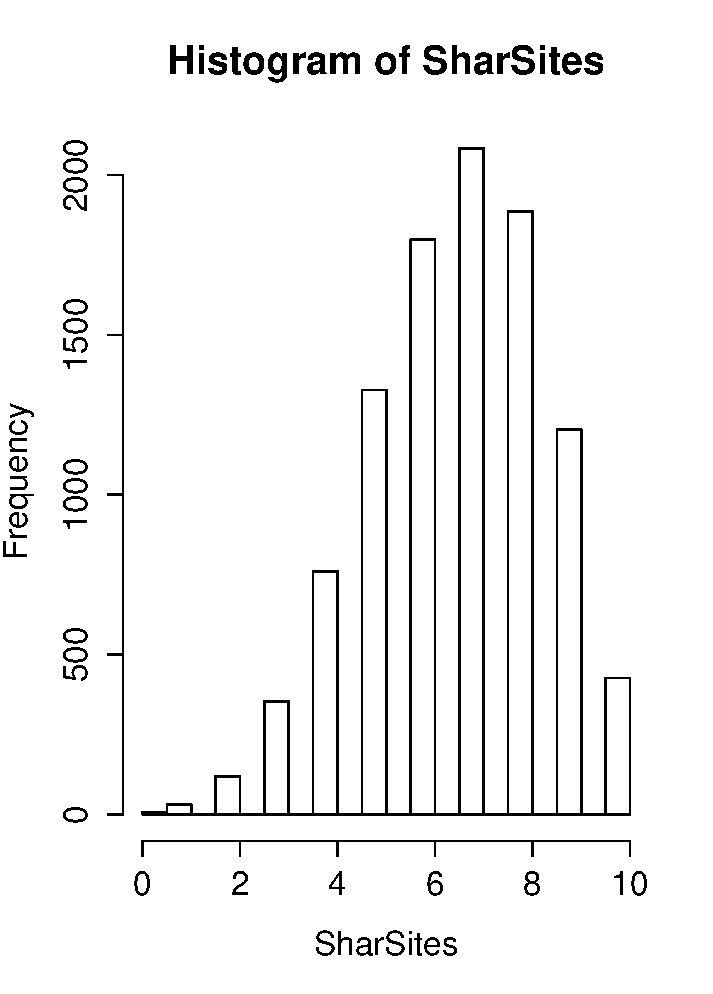
\includegraphics[width=.5\textwidth]{Figures/Ne200Hist.pdf}
    \caption{Histogram of the number of shared segregating sites for $N_e = 200$. }\label{fig:SegSites}
\end{figure}


3. Repeat that same experiment for values of Ne = 25, 50, 100, 500, 1000, 5000, and 50000.\\
It has now become apparent that earlier assumptions that I have made are wrong, because 
irrespective of the effective population size, I will get the same answer. 
Ok, I don't really have that much time left. So I will look at $N_e$ of 25 and 50,000. 

\begin{figure}
\centering
     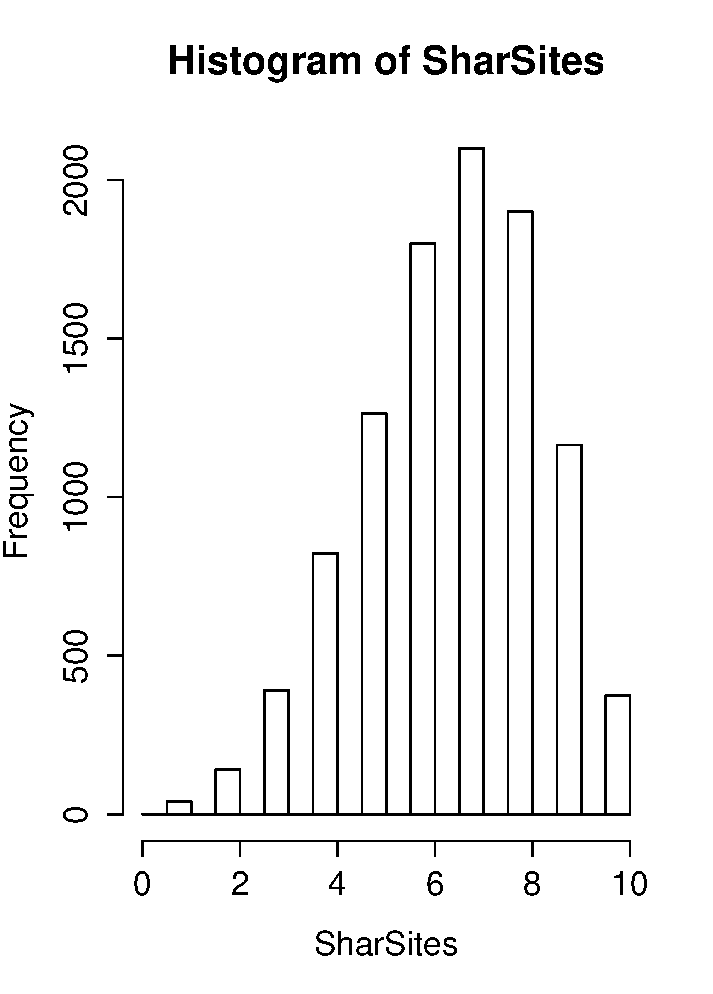
\includegraphics[width=.5\textwidth]{Figures/Ne25Hist.pdf}
    \caption{Histogram of the number of shared segregating sites for $N_e = 200$. }\label{fig:SegSites}
\end{figure}

\begin{figure}
\centering
     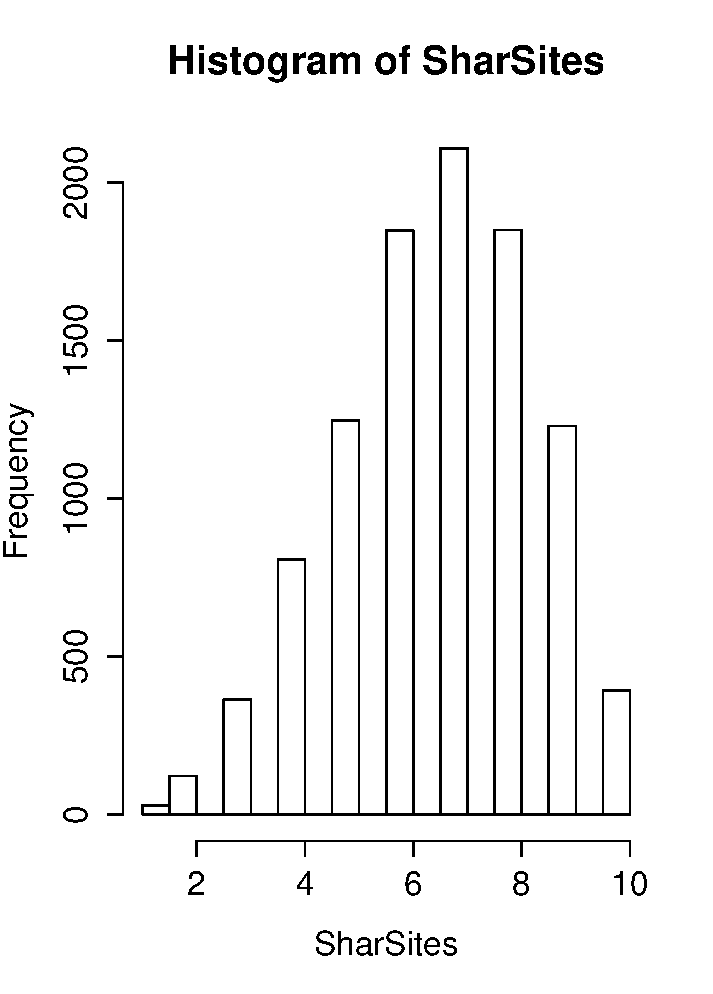
\includegraphics[width=.5\textwidth]{Figures/Ne50000Hist.pdf}
    \caption{Histogram of the number of shared segregating sites for $N_e = 200$. }\label{fig:SegSites}
\end{figure}

It appears, that I am not parameterizing my model correctly as all three graphs are very similar.

4. What is going on here? Draw a picture (you can draw it and annotate it in pen, if desired, and shoot a picture of it with you smart phone) of these scenarios in terms of the coalescent and discuss the importance of tree length ancestral to both populations. Even with very large Ne the proportion of shared polymorphisms in the two samples never approaches 1. Why?\\

5. What if you wanted to simulate microsatellite data from the coalescent? There is a perl script called ms2ms that does this, as well as the program that we have used, called ms2geno. Describe in your own words how the sequence output of ms is used by ms2ms or ms2geno to simulate microsatellites.\\

As I understand it the program ms uses an infinite sites model for mutation. In this model, each mutation produces a new
polymorphism. Hudson suggests in his manual that the output of the gene tree can be then used by other
programs to evolve them under a different model. Microsatellites are characterized by a stepwise mutational model
where alleles are represented by an integer value and mutation results in either an increase or decrease in the 
integer (i.e. for a dinucleotide microsatellite it can either gain or lose two bases). So it seems reasonable that if we were 
to look at the above simulated sequences we have produced 10 different non-recombining segregating sites. 
Each 0 means that an individual inherited the ancestral copy and a 1 means they received a copy that had
mutated from the ancestral type. 


\bibliographystyle{men}
\bibliography{CompsCoal}

\end{document}  